\newpage
%\section{Results}
\chapter{Results}
\label{sec:results}
\section{Evaluation of Anomaly detectors}
To evaluate the performance of the anomaly detectors described in section \ref{sec:anomaly_detectors_theory}, tests on real hyperspectral data from the Cuprite scene was done in MATLAB as described in section \ref{sec:MATLAB_methodology}. Band 220 from the Cuprite scene can be seen in figure \ref{fig:cuprite_scene_band_220}.

\begin{figure}[H]

\hbox{\hspace*{-2cm}                                                           

   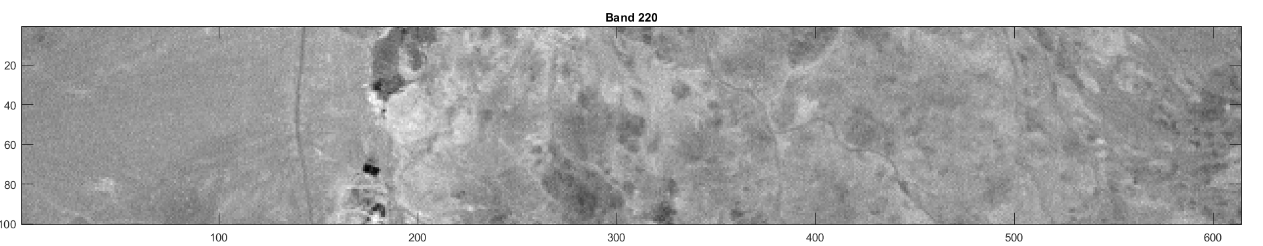
\includegraphics[scale=0.3]{images/AD_testing/original_band_220_22_1.png}}
  \caption{Spectral band 220 from the hyperspectral data set of the Cuprite site\cite{Cuprite_data}. } 
  \label{fig:cuprite_scene_band_220}
\end{figure}



\subsection{RX}

\begin{figure}[H]

\hbox{\hspace*{-2cm}                                                           

   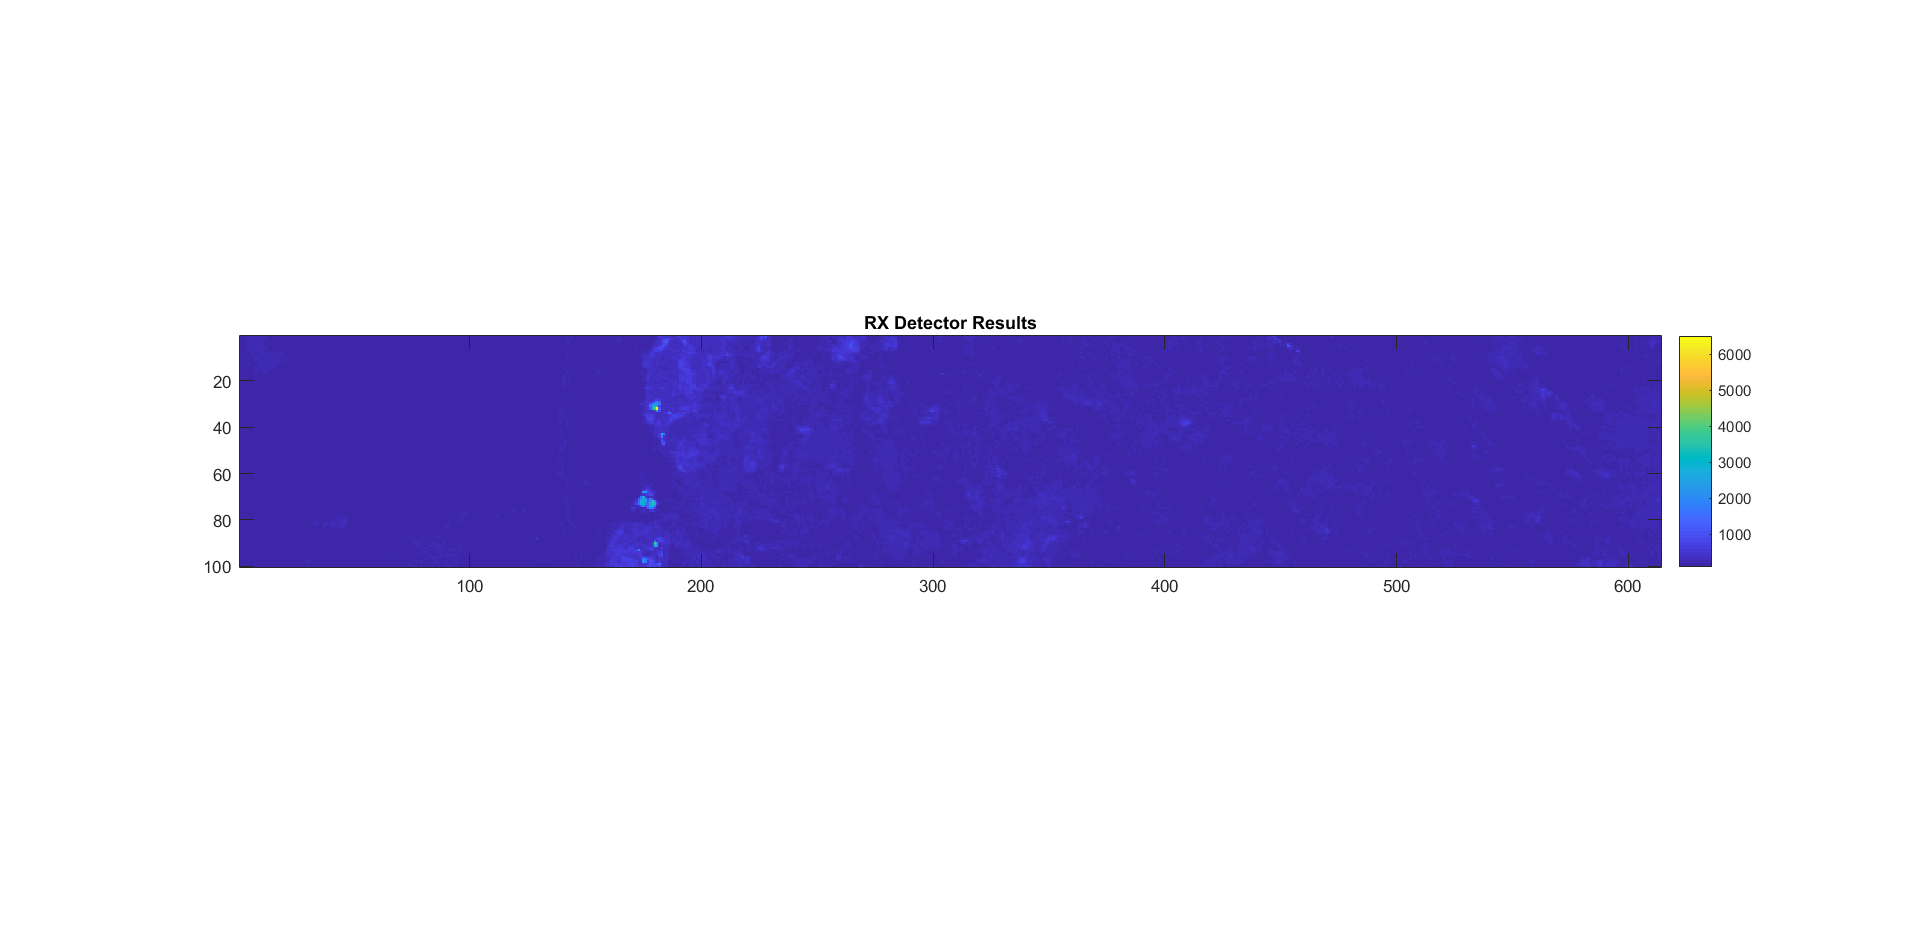
\includegraphics[scale=0.4]{images/AD_testing/GRX_22_1.png}}
  \caption{Result from RX AD on Cuprite image data. } 
  \label{fig:cuprite_scene_band_220}
\end{figure}


\subsection{LRX}

\begin{figure}[H]

\hbox{\hspace*{-2cm}                                                           

   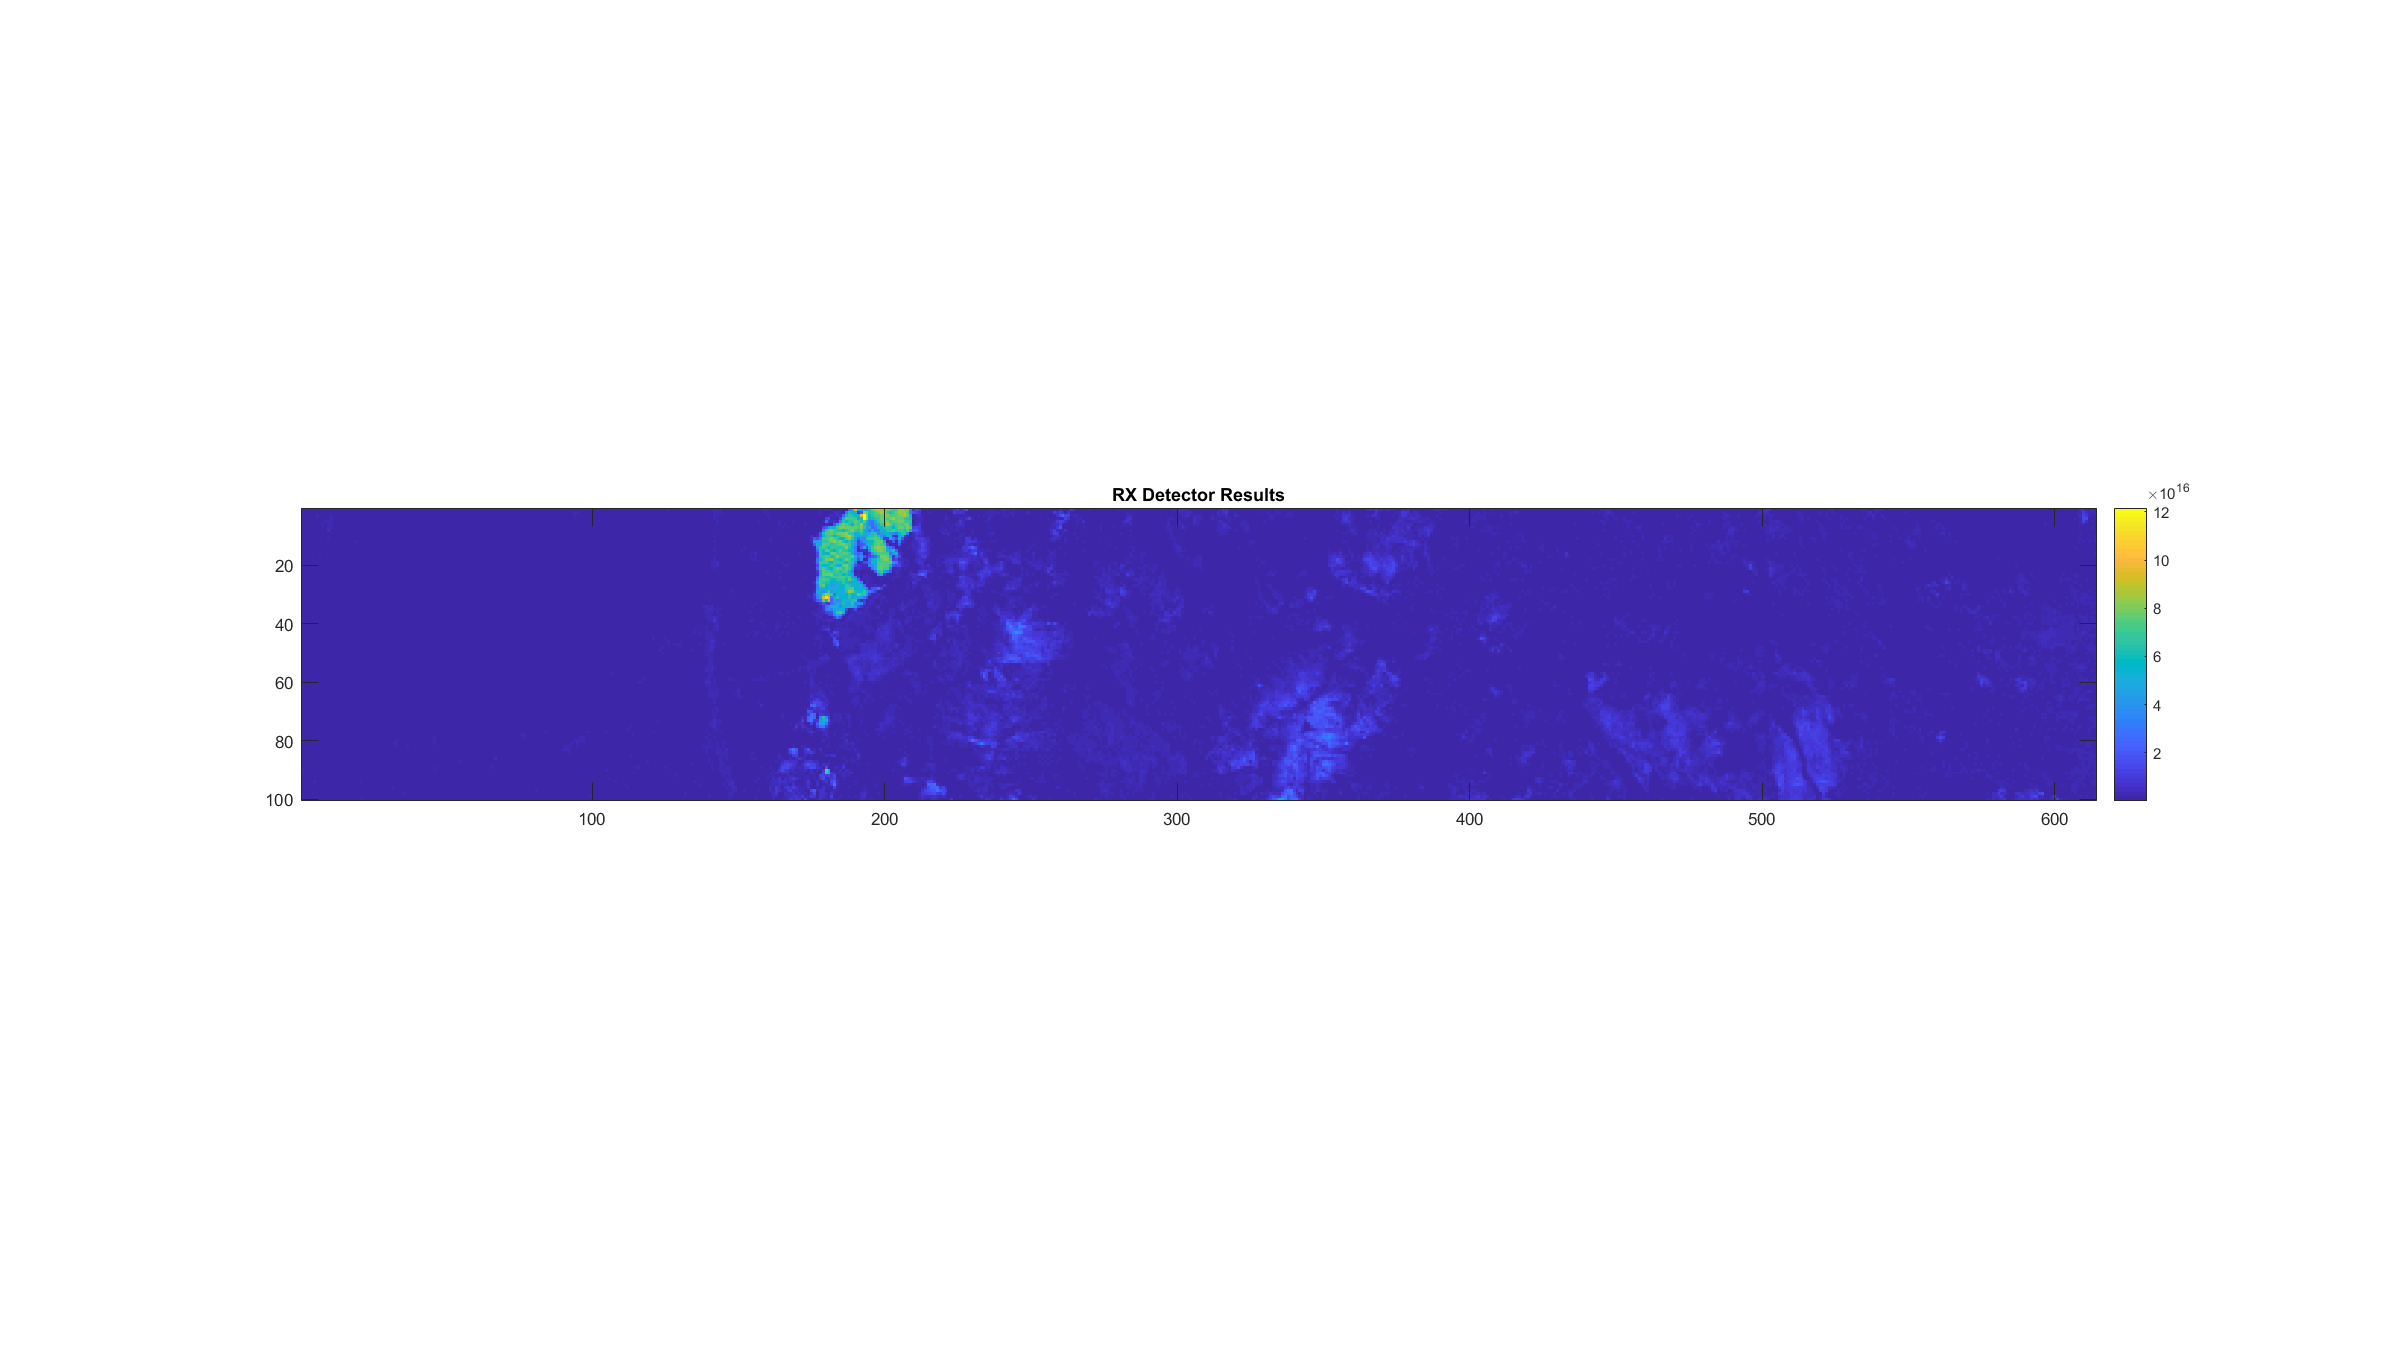
\includegraphics[scale=0.3]{images/AD_testing/K=23.png}}
  \caption{Result from LRX AD with a kernel size of K=23 on Cuprite image data. } 
  \label{fig:cuprite_scene_band_220}
\end{figure}


\subsection{ACAD}

\begin{figure}[H]
\centering                                                           

   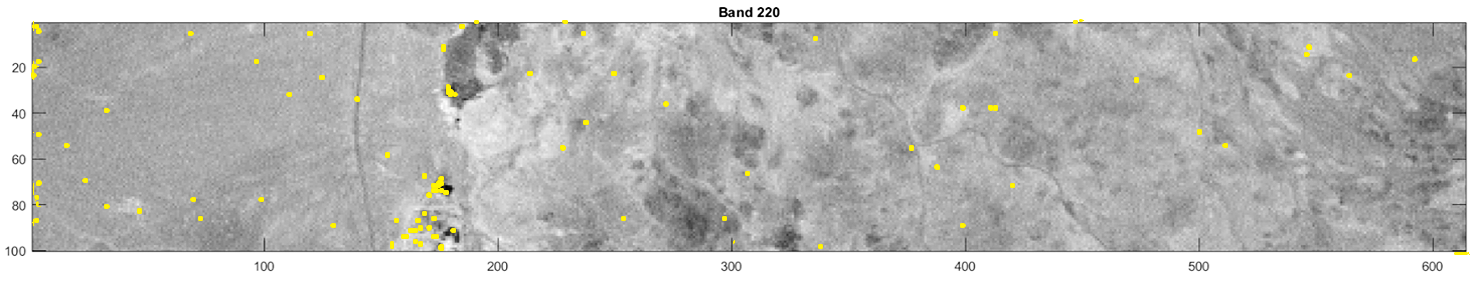
\includegraphics[scale=0.3]{images/AD_testing/anomaly_map_over_picture_tresh=250.png}
  \caption{Anomaly map created by ACAD( yellow dots) overlayed over Figure \ref{fig:cuprite_scene_band_220}. $\tau$ is set to 250.} 
  \label{fig:cuprite_scene_band_220}
\end{figure}

